\chapter{Mengenal Kecerdasan Buatan dan Scikit-Learn}
Buku umum teori lengkap yang digunakan memiliki judul\textit{Artificial intelligence: a modern approach}\cite{russell2016artificial}.  
Untuk pratikum sebelum UTS menggunakan buku \textit{Python Artificial Intelligence Projects for Beginners}\cite{eckroth2018python}. Buku pelengkap penunjang penggunaan python menggunakan buku \textit{Python code for Artificial Intelligence: Foundations of Computational Agents}\cite{poole2017python}.
Dengan praktek menggunakan python 3 dan editor anaconda dan library python scikit-learn.
Tujuan pembelajaran pada pertemuan pertama antara lain:
\begin{enumerate}
\item
Mengerti definisi kecerdasan buatan, sejarah kecerdasan buatan, perkembangan dan penggunaan di perusahaan
\item
Memahami cara instalasi dan pemakaian sci-kit learn
\item
Memahami cara penggunaan variabel explorer di spyder
\end{enumerate}
Tugas dengan cara dikumpulkan dengan pull request ke github dengan menggunakan latex pada repo yang dibuat oleh asisten riset.

\section{Teori}
Praktek teori penunjang yang dikerjakan :
\begin{enumerate}
\item
Definisi Sejarah serta Perkembangan Kecerdasan Buatan\\
Definisi dari Kecerdasan buatan adalah suatu teknologi yang terdapat pada bidang ilmu komputer yang dapat melakukan manipulasi kecerdasan manusia yang dimasukkan pada mesin agar dapat menyelesaikan persoalan dan pekerjaan seperti yang dilakukan oleh manusia atau mungkin dapat lebih baik dari manusia. Adapun sejarah dari kecerdasan buatan atau dapat disebut Artificial Intelligence bermula ketika munculna komputer pada tahun 1940 pada saat itu banyak sekali perhatian yang dapat difokuskan pada kemampuan komputer dalam mengerjakan sesuatu yang dapat dilakukan oleh manusia. komputer dapat menirukan kemampuan kecerdasan dan perilaku manusia. pada tahun 1956 ilmuan seperti Alan Turing, Norbert Wiener dan yang lainnya melakukan kerja sama dalam beberapa ilmu seorang ilmuan memdapatkan suatu ide untuk membuat kecerdasan buatan sehingga suatu kecerdasan tersebut dibuat agar dapat meniru perilaku manusia. adapun perkembangan dari kecerdasan buatan yaitu pada saat ini banyak sekali jenis mesin yang dapat berperilaku layaknya manusia dengan beragam kemampuan yang diberikan contohnya yaitu google assistant.
\item
Supervised Learning dan Unsupervised Learning\\
Supervised Learning adalah suatu pembelajaran yang didalamnya terdapat pengawas atau dapat diartikan supervisor. Supervisor merupakan suatu label yang ada di setiap data nya. Kemudian label tersebut berisi tag dari data yang ditambahkan kedalam model pembelajaran mesin atau lebih trend disebut dengan machine learning model. Unsupervised Learning Merupakan suaru pembelajaran tanpa adanya sebuah pengawasan dan tidak menggunakan label untuk bisa memprediksi target variabel\\
\item
Klasifikasi dan Regresi\\
Klasifikasi merupakan sampel yang dimiliki oleh dua atau lebih kelas yang dikelompokkan yang disesuaikan berdasarkan ukuran kemiripan atau jarak yang melekat.Regresi merupakan sebuah predikasi apabila hasil atau output yang diinginkan terdiri dari satu atau lebih variabel. Teknik klasifikasi menyediakan model atau fungsi prediktif yang memprediksi data baru dalam kategori atau label tersendiri dengan bantuan data historis. Sebaliknya, metode regresi memodelkan fungsi bernilai kontinu yang berarti memprediksi data dalam data numerik kontinu.\\
\item
Dataset Training set dan Testing set\\
Dataset merupakan kumpulan objek yang merepresentasikan data dan juga relasi yang ada di memory yang bersifat homogen. Trainingset Merupakan sebuah data yang digunakan untuk melakukan klasifikasi ataupun prediksi. Dengan adanya data training maka akan didapatkan sebuah model regresi. Testingset Digunakan untuk menguji kebenaran dari sebuah model data.yang berisi unseen example merupakan contoh yang tidak ada didalam trainingset.
\end{enumerate}

\section{Instalasi}
Membuka https://scikit-learn.org/stable/tutorial/basic/tutorial.html. Dengan menggunakan bahasa yang mudah dimengerti dan bebas plagiat. 
Dan wajib skrinsut dari komputer sendiri.
\begin{enumerate}
\item
Instalasi library scikit dari anaconda, mencoba kompilasi dan uji coba ambil contoh kode dan lihat variabel explorer[hari ke 1](10)
\begin{figure}[!htbp]
		\centering
		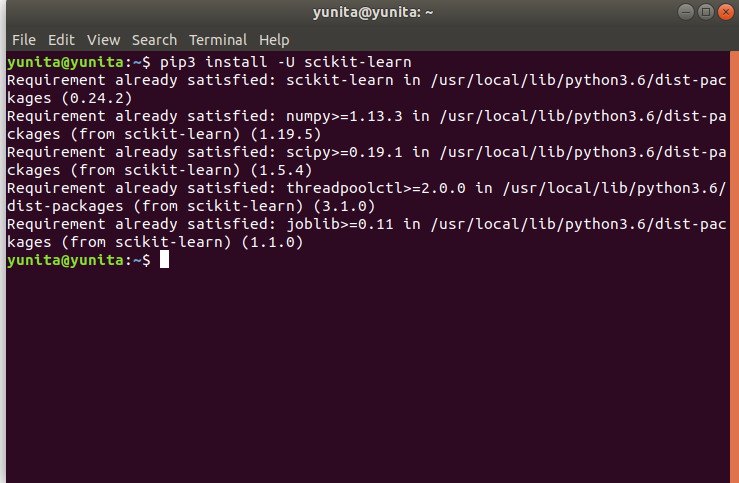
\includegraphics[scale=0.4]{figures/1.PNG}
		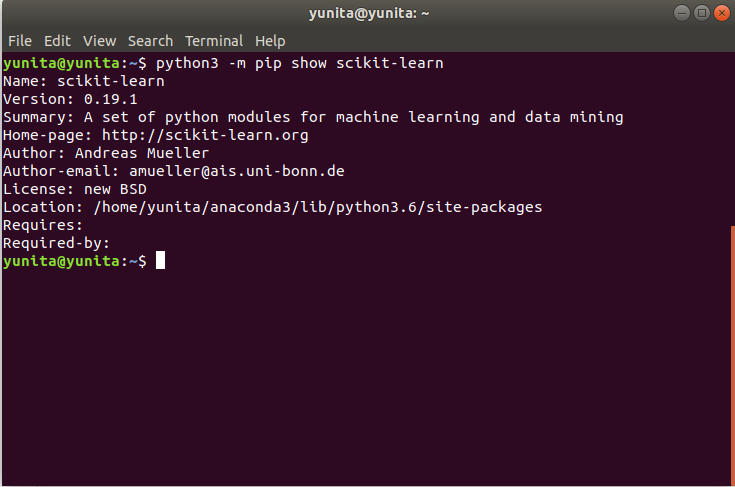
\includegraphics[scale=0.5]{figures/2.PNG}
	\end{figure}
\newpage
\item
Mencoba Loading an example dataset, menjelaskan maksud dari tulisan tersebut dan mengartikan per baris[hari ke 1](10)
\begin{figure}[!htbp]
		\centering
		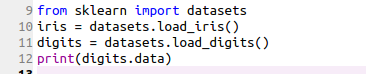
\includegraphics[scale=0.4]{figures/3.PNG}
		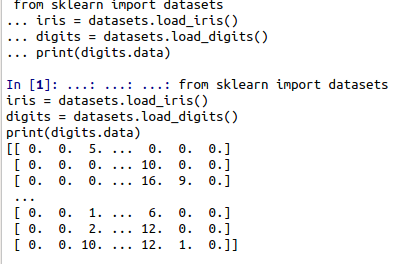
\includegraphics[scale=0.5]{figures/4.PNG}
	\end{figure}
\newpage
\item
Mencoba Learning and predicting, menjelaskan maksud dari tulisan tersebut dan mengartikan per baris[hari ke 2](10)
\begin{figure}[!htbp]
		\centering
		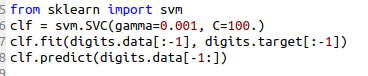
\includegraphics[scale=0.4]{figures/5.PNG}
		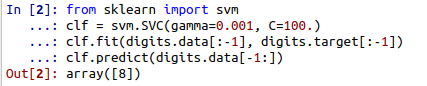
\includegraphics[scale=0.5]{figures/6.PNG}
	\end{figure}
\newpage
\item
mencoba Model persistence, menjelaskan maksud dari tulisan tersebut dan mengartikan per baris[hari ke 2](10)
\begin{figure}[!htbp]
		\centering
		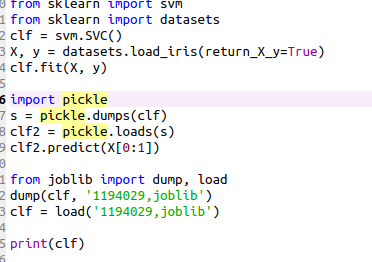
\includegraphics[scale=0.4]{figures/7.PNG}
		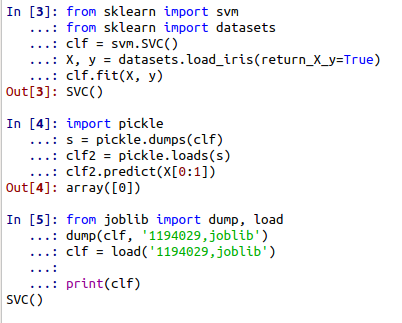
\includegraphics[scale=0.5]{figures/8.PNG}
	\end{figure}
\newpage
\item 
Mencoba Conventions, menjelaskan maksud dari tulisan tersebut dan mengartikan per baris[hari ke 2](10)
\begin{figure}[!htbp]
		\centering
		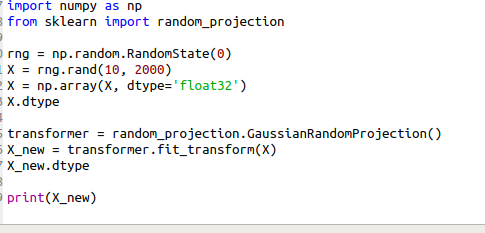
\includegraphics[scale=0.4]{figures/9.PNG}
		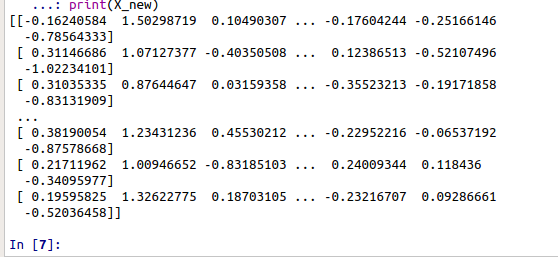
\includegraphics[scale=0.5]{figures/10.PNG}
	\end{figure}
\newpage
\end{enumerate}


\section{Penanganan Error}
Dari percobaan yang dilakukan di atas, apabila mendapatkan error maka:

\begin{enumerate}
	\item
	skrinsut error[hari ke 2](10)
	\item
Tuliskan kode eror dan jenis errornya [hari ke 2](10)
	\item
Solusi pemecahan masalah error tersebut[hari ke 2](10)

\end{enumerate}

